\documentclass[pdf]{beamer}
\mode<presentation>{}
\usepackage{minted}
\usepackage{tikz}
\usepackage{pgffor} %% gives looping with \foreach
\usepackage[absolute,overlay]{textpos}
\usepackage{lmodern} %% scalable latin characters
\usetikzlibrary{arrows,shapes,backgrounds}
\usepackage{multirow}
\usepackage{listings} %% another package for code related stuff


%% stuff for minted
\definecolor{mintedBg}{rgb}{0.95, 0.95, 0.95}
\definecolor{blockBg}{rgb}{0.6, 0.6, 0.95}
\definecolor{rnaColor}{rgb}{0, 0.6, 0}
\definecolor{cdsColor}{rgb}{0, 0.4, 0.4}
\definecolor{rnaPol}{rgb}{0.8,0,0.8}
\definecolor{ribosomeCol}{rgb}{0.5,0.5,0.1}
\definecolor{protColor}{rgb}{0.6,0,0.6}
%% colours for nucleotides:
\definecolor{dACol}{rgb}{0.5, 0.5, 0}
\definecolor{dCCol}{rgb}{0.8, 0, 0}
\definecolor{dGCol}{rgb}{0, 0.8, 0}
\definecolor{dTCol}{rgb}{0, 0, 0.8}

\definecolor{navy}{rgb}{0, 0, 0.6}
\definecolor{pur}{rgb}{0, 0, 0.6}
\definecolor{pyr}{rgb}{0.6, 0, 0.2}
%% define styles for different codes
\newminted{cpp}{linenos, bgcolor=mintedBg, fontsize=\footnotesize}
%% then use \begin{cppcode}
\newminted{c}{linenos, bgcolor=mintedBg, fontsize=\footnotesize}
\newminted{perl}{linenos, bgcolor=mintedBg, fontsize=\tiny}
\newminted{sh}{linenos, bgcolor=mintedBg, fontsize=\footnotesize,
  language=bash}
\newminted{console}{linenos, bgcolor=mintedBg, fontsize=\footnotesize}

%% a command to define a subheading
\newcommand\subHeading[1]{
  \par\bigskip {\Large\bfseries#1}\par\smallskip
}

%% I detest indentation in footnotes etc, so try this:
\makeatletter
\renewcommand\@makefntext[1]{\noindent\makebox[0em][r]{\@makefnmark}\tiny#1}
\makeatother
%% the makeatletter and makeatother are required to allow me to
%% to change the macro beginning with an @. (though when I call it
%% I don't use the @ ... 

\setlength\parskip{0.5em}
\setlength\parindent{0ex}

%% to have footnotes without references. This from tex.stackexchange.com
\newcommand\blfootnote[1]{%
  \begingroup  %% this makes it a local redefinition
  \renewcommand\thefootnote{}\footnote{#1}%
  \addtocounter{footnote}{-1}  % this adjusts the footnote counter
  \endgroup
}


\title{Implementing dynamic programming in Perl}
\subtitle{Optimal alignment}
\author{Martin Jakt}

\begin{document}

\begin{frame}
  \titlepage
\end{frame}


\begin{frame}{Needleman-Wunsch: global alignment}
  \begin{figure}[ht]
    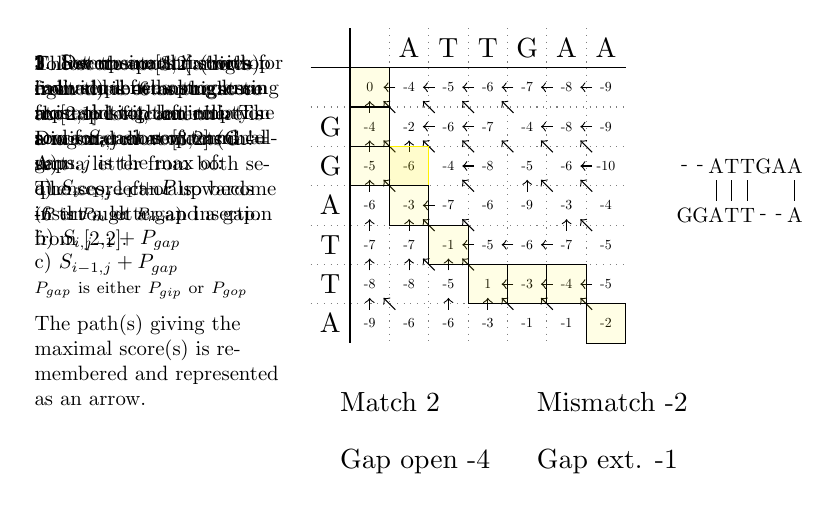
\begin{tikzpicture}[scale=0.5]
      \node [right] at (1,-1) {Match 2};
\node [right] at (6,-1) {Mismatch -2};
\node [right] at (1,-2.5) {Gap open -4};
\node [right] at (6,-2.5) {Gap ext. -1};

\draw [-] (0.5,7.5) -- (8.5,7.5);
\draw [-] (1.5,8.5) -- (1.5,0.5);
\draw [-, dotted, opacity=0.5] (0.5,6.5) -- (8.5,6.5);
\draw [-, dotted, opacity=0.5] (2.5,8.5) -- (2.5,0.5);
	\node at (3,8) {A};
	\draw [-, dotted, opacity=0.5] (3.5,8.5) -- (3.5,0.5);
	\node at (4,8) {T};
	\draw [-, dotted, opacity=0.5] (4.5,8.5) -- (4.5,0.5);
	\node at (5,8) {T};
	\draw [-, dotted, opacity=0.5] (5.5,8.5) -- (5.5,0.5);
	\node at (6,8) {G};
	\draw [-, dotted, opacity=0.5] (6.5,8.5) -- (6.5,0.5);
	\node at (7,8) {A};
	\draw [-, dotted, opacity=0.5] (7.5,8.5) -- (7.5,0.5);
	\node at (8,8) {A};
	\node at (1,6) {G};
	\draw [-, dotted, opacity=0.5] (0.5,5.5) -- (8.5,5.5);
	\node at (1,5) {G};
	\draw [-, dotted, opacity=0.5] (0.5,4.5) -- (8.5,4.5);
	\node at (1,4) {A};
	\draw [-, dotted, opacity=0.5] (0.5,3.5) -- (8.5,3.5);
	\node at (1,3) {T};
	\draw [-, dotted, opacity=0.5] (0.5,2.5) -- (8.5,2.5);
	\node at (1,2) {T};
	\draw [-, dotted, opacity=0.5] (0.5,1.5) -- (8.5,1.5);
	\node at (1,1) {A};



	\node [below left, align=left, scale=0.75, text width=12em] 
	at (0,8) {1. Set up a matrix with each sequence 
	along an axis and with an empty row for each sequence.};



	\node[scale=0.5] at (2,7) {0};
	\node[scale=0.5] at (3,7) {-4};
	\draw [->] (2.65, 6+1) -- (2.35, 6+1);
	\node[scale=0.5] at(4,7) {-5};
	\draw [->] (3.65,6+1) -- (3.35,6+1);
	\node[scale=0.5] at(5,7) {-6};
	\draw [->] (4.65,6+1) -- (4.35,6+1);
	\node[scale=0.5] at(6,7) {-7};
	\draw [->] (5.65,6+1) -- (5.35,6+1);
	\node[scale=0.5] at(7,7) {-8};
	\draw [->] (6.65,6+1) -- (6.35,6+1);
	\node[scale=0.5] at(8,7) {-9};
	\draw [->] (7.65,6+1) -- (7.35,6+1);
	\node[scale=0.5] at (2,6) {-4};
	\draw [->] (2,6 + 0.35) -- (2, 6 + 0.65);
	\node[scale=0.5] at(2,5) {-5};
	\draw [->] (2,6-1 + 0.35) -- (2, 6-1 + 0.65);
	\node[scale=0.5] at(2,4) {-6};
	\draw [->] (2,6-2 + 0.35) -- (2, 6-2 + 0.65);
	\node[scale=0.5] at(2,3) {-7};
	\draw [->] (2,6-3 + 0.35) -- (2, 6-3 + 0.65);
	\node[scale=0.5] at(2,2) {-8};
	\draw [->] (2,6-4 + 0.35) -- (2, 6-4 + 0.65);
	\node[scale=0.5] at(2,1) {-9};
	\draw [->] (2,6-5 + 0.35) -- (2, 6-5 + 0.65);



	\node [below left, align=left, scale=0.75, text width=12em] 
	at (0,8) {2. Insert scores in the top row and left-most column representing
	the initiation and extension of terminal gaps.};



	\node [scale=0.5] at (3,6) {-2};
	\draw [->] (2.65,6.35) -- (2.35,6.65);
	\node [scale=0.5] at (4,6) {-6};
	\draw [->] (3.65,6.35) -- (3.35,6.65);
	\draw [->] (3.65,6) -- (3.35,6);
	\node [scale=0.5] at (5,6) {-7};
	\draw [->] (4.65,6.35) -- (4.35,6.65);
	\draw [->] (4.65,6) -- (4.35,6);
	\node [scale=0.5] at (6,6) {-4};
	\draw [->] (5.65,6.35) -- (5.35,6.65);
	\node [scale=0.5] at (7,6) {-8};
	\draw [->] (6.65,6) -- (6.35,6);
	\node [scale=0.5] at (8,6) {-9};
	\draw [->] (7.65,6) -- (7.35,6);



	\node [below left, align=left, scale=0.75, text width=12em] 
	at (0,8) {3. Determine the scores for individual cells progressing from
	the top left cell. The score $S_{i,j}$ at row $i$ and column $j$ is the max of:\\
	a) $S_{i-1,j-1} + P$\\
	{\footnotesize($P$ is $P_m$ or $P_{mm}$).
	}\\
	b) $S_{i,j-1} + P_{gap}$\\
	c) $S_{i-1,j} + P_{gap}$\\
	{\footnotesize $P_{gap}$ is either $P_{gip}$ or $P_{gop}$}\\
	\vspace{0.2cm}
	The path(s) giving the maximal score(s) is remembered and represented as
	an arrow.
	};




	\node [scale=0.5] at (3,5) {-6};
	\draw [->] (2.65,5.35) -- (2.35,5.65);
	\draw [->] (3,5.35) -- (3,5.65);
	\node [scale=0.5] at (4,5) {-4};
	\draw [->] (3.65,5.35) -- (3.35,5.65);
	\node [scale=0.5] at (5,5) {-8};
	\draw [->] (4.65,5.35) -- (4.35,5.65);
	\draw [->] (4.65,5) -- (4.35,5);
	\node [scale=0.5] at (6,5) {-5};
	\draw [->] (5.65,5.35) -- (5.35,5.65);
	\node [scale=0.5] at (7,5) {-6};
	\draw [->] (6.65,5.35) -- (6.35,5.65);
	\node [scale=0.5] at (8,5) {-10};
	\draw [->] (7.65,5.35) -- (7.35,5.65);
	\draw [->] (7.65,5) -- (7.35,5);



	\draw [fill, yellow, fill opacity=0.2] (2.5,4.5) rectangle (3.5,5.5);
	\node [below left, align=left, scale=0.75, text width=12em] 
	at (0,8) {
	The score at [3,2] (highlighted) is -6 as the score at [2,1] is -4, and there is a
	mismatch at [3,2] (G != A). 

	The score can also become -6 through a gap
	insertion from [2,2].
	};




	\node [scale=0.5] at (3,4) {-3};
	\draw [->] (2.65,4.35) -- (2.35,4.65);
	\node [scale=0.5] at (4,4) {-7};
	\draw [->] (3.65,4) -- (3.35,4);
	\node [scale=0.5] at (5,4) {-6};
	\draw [->] (4.65,4.35) -- (4.35,4.65);
	\node [scale=0.5] at (6,4) {-9};
	\draw [->] (6,4.35) -- (6,4.65);
	\node [scale=0.5] at (7,4) {-3};
	\draw [->] (6.65,4.35) -- (6.35,4.65);
	\node [scale=0.5] at (8,4) {-4};
	\draw [->] (7.65,4.35) -- (7.35,4.65);


	\node [scale=0.5] at (3,3) {-7};
	\draw [->] (3,3.35) -- (3,3.65);
	\node [scale=0.5] at (4,3) {-1};
	\draw [->] (3.65,3.35) -- (3.35,3.65);
	\node [scale=0.5] at (5,3) {-5};
	\draw [->] (4.65,3.35) -- (4.35,3.65);
	\draw [->] (4.65,3) -- (4.35,3);
	\node [scale=0.5] at (6,3) {-6};
	\draw [->] (5.65,3) -- (5.35,3);
	\node [scale=0.5] at (7,3) {-7};
	\draw [->] (6.65,3) -- (6.35,3);
	\draw [->] (7,3.35) -- (7,3.65);
	\node [scale=0.5] at (8,3) {-5};
	\draw [->] (7.65,3.35) -- (7.35,3.65);


	\node [scale=0.5] at (3,2) {-8};
	\draw [->] (3,2.35) -- (3,2.65);
	\node [scale=0.5] at (4,2) {-5};
	\draw [->] (3.65,2.35) -- (3.35,2.65);
	\draw [->] (4,2.35) -- (4,2.65);
	\node [scale=0.5] at (5,2) {1};
	\draw [->] (4.65,2.35) -- (4.35,2.65);
	\node [scale=0.5] at (6,2) {-3};
	\draw [->] (5.65,2) -- (5.35,2);
	\node [scale=0.5] at (7,2) {-4};
	\draw [->] (6.65,2) -- (6.35,2);
	\node [scale=0.5] at (8,2) {-5};
	\draw [->] (7.65,2) -- (7.35,2);


	\node [scale=0.5] at (3,1) {-6};
	\draw [->] (2.65,1.35) -- (2.35,1.65);
	\node [scale=0.5] at (4,1) {-6};
	\draw [->] (4,1.35) -- (4,1.65);
	\node [scale=0.5] at (5,1) {-3};
	\draw [->] (5,1.35) -- (5,1.65);
	\node [scale=0.5] at (6,1) {-1};
	\draw [->] (5.65,1.35) -- (5.35,1.65);
	\node [scale=0.5] at (7,1) {-1};
	\draw [->] (6.65,1.35) -- (6.35,1.65);
	\node [scale=0.5] at (8,1) {-2};
	\draw [->] (7.65,1.35) -- (7.35,1.65);

\draw [fill=yellow, fill opacity=0.1] (7.5,0.5) rectangle (8.5,1.5);


\draw [fill=yellow, fill opacity=0.1] (6.5,1.5) rectangle (7.5,2.5);


\draw [fill=yellow, fill opacity=0.1] (5.5,1.5) rectangle (6.5,2.5);


\draw [fill=yellow, fill opacity=0.1] (4.5,1.5) rectangle (5.5,2.5);


\draw [fill=yellow, fill opacity=0.1] (3.5,2.5) rectangle (4.5,3.5);


\draw [fill=yellow, fill opacity=0.1] (2.5,3.5) rectangle (3.5,4.5);


\draw [fill=yellow, fill opacity=0.1] (1.5,4.5) rectangle (2.5,5.5);


\draw [fill=yellow, fill opacity=0.1] (1.5,5.5) rectangle (2.5,6.5);


\draw [fill=yellow, fill opacity=0.1] (1.5,6.5) rectangle (2.5,7.5);



	\node [below left, align=left, scale=0.75, text width=12em] 
	at (0,8) {
	Follow the path (arrows) from the bottom right to
	the top left corner.

	Diagonal movements insert a letter from both sequences,
	left or upwards insert a letter and a gap.
	};



\node [scale=0.75] (s1) at (10 + 0/2.5, 5) {-};
\node [scale=0.75] (s2) at (10 + 0/2.5, 5-1.25) {G};
\node [scale=0.75] (s1) at (10 + 1/2.5, 5) {-};
\node [scale=0.75] (s2) at (10 + 1/2.5, 5-1.25) {G};
\node [scale=0.75] (s1) at (10 + 2/2.5, 5) {A};
\node [scale=0.75] (s2) at (10 + 2/2.5, 5-1.25) {A};
\draw [-] (s1) -- (s2);
\node [scale=0.75] (s1) at (10 + 3/2.5, 5) {T};
\node [scale=0.75] (s2) at (10 + 3/2.5, 5-1.25) {T};
\draw [-] (s1) -- (s2);
\node [scale=0.75] (s1) at (10 + 4/2.5, 5) {T};
\node [scale=0.75] (s2) at (10 + 4/2.5, 5-1.25) {T};
\draw [-] (s1) -- (s2);
\node [scale=0.75] (s1) at (10 + 5/2.5, 5) {G};
\node [scale=0.75] (s2) at (10 + 5/2.5, 5-1.25) {-};
\node [scale=0.75] (s1) at (10 + 6/2.5, 5) {A};
\node [scale=0.75] (s2) at (10 + 6/2.5, 5-1.25) {-};
\node [scale=0.75] (s1) at (10 + 7/2.5, 5) {A};
\node [scale=0.75] (s2) at (10 + 7/2.5, 5-1.25) {A};
\draw [-] (s1) -- (s2);


    \end{tikzpicture}
  \end{figure}
\end{frame}

\begin{frame}[fragile]{Where to start?}
  \footnotesize{
  Data and how to represent it:
  \begin{itemize}
  \item sequences from file $\rightarrow$ strings
  \item a scoring system
    \footnotesize{
    \begin{itemize}
      \item If DNA sequence, from the command line?\\
        Scalar variables: \verb|$match|, \verb|$mismatch|, \verb|$mismatch|,
        \verb|$gap_open|, \verb|$gap_extend|.
      \item If protein sequences we need a scoring matrix.\\
        Two dimensional hash: \verb|$matrix{aa1}{aa2}|
    \end{itemize}
    }
  \item A table to hold the scores:\\
    Two dimensional array: \verb|$scores[$i][$j]|
  \item A table to hold the arrows:\\
    Two dimensional array: \verb|$pointers[$i][$j]|\\
    but how???
  \item Something to represent one or more alignments?\\
    Various options, we'll work it out later...
  \end{itemize}
}
\end{frame}

\begin{frame}[fragile]{The structure of the script (functions)}
  Functions:
  \begin{itemize}
  \item A sequence read function
  \item A matrix read function (if we do proteins)
  \item An function to initiate the scoring and pointer matrices
  \item A scoring function (determines score and pointer direction for a
    single cell of the table)
  \item A function to trace back the optimal alignment or alignments.
  \end{itemize}
\end{frame}

\begin{frame}[fragile]{The structure of the script (order)}
  \begin{enumerate}
  \item Process command line:\\
    eg. get input files, and maybe some scoring parameters
  \item Read in sequences
  \item Read in substitution matrix
  \item Initialise the scoring and pointer matrices
  \item Determine the scores and recored the pointers
  \item Traceback the alignment
  \end{enumerate}
\end{frame}

\begin{frame}[fragile]{Initialise the score and pointer tables}
  \begin{figure}[ht]
    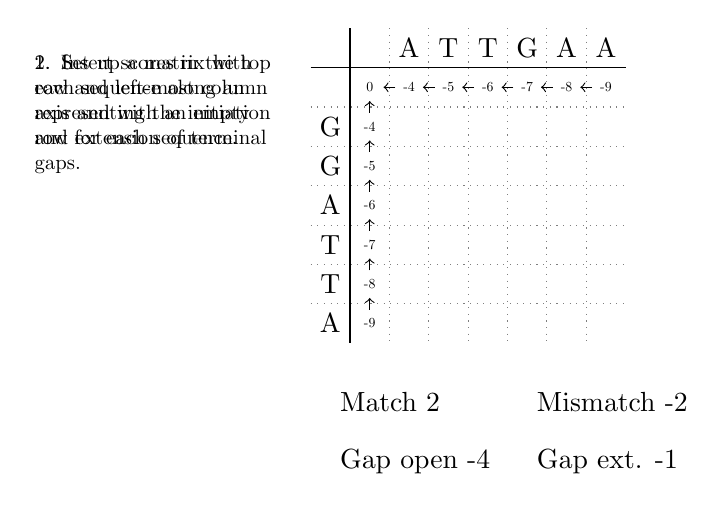
\begin{tikzpicture}[scale=0.5]
      \node [right] at (1,-1) {Match 2};
\node [right] at (6,-1) {Mismatch -2};
\node [right] at (1,-2.5) {Gap open -4};
\node [right] at (6,-2.5) {Gap ext. -1};
\visible<1->{
\draw [-] (0.5,7.5) -- (8.5,7.5);
\draw [-] (1.5,8.5) -- (1.5,0.5);
\draw [-, dotted, opacity=0.5] (0.5,6.5) -- (8.5,6.5);
\draw [-, dotted, opacity=0.5] (2.5,8.5) -- (2.5,0.5);
	\node at (3,8) {A};
	\draw [-, dotted, opacity=0.5] (3.5,8.5) -- (3.5,0.5);
	\node at (4,8) {T};
	\draw [-, dotted, opacity=0.5] (4.5,8.5) -- (4.5,0.5);
	\node at (5,8) {T};
	\draw [-, dotted, opacity=0.5] (5.5,8.5) -- (5.5,0.5);
	\node at (6,8) {G};
	\draw [-, dotted, opacity=0.5] (6.5,8.5) -- (6.5,0.5);
	\node at (7,8) {A};
	\draw [-, dotted, opacity=0.5] (7.5,8.5) -- (7.5,0.5);
	\node at (8,8) {A};
	\node at (1,6) {G};
	\draw [-, dotted, opacity=0.5] (0.5,5.5) -- (8.5,5.5);
	\node at (1,5) {G};
	\draw [-, dotted, opacity=0.5] (0.5,4.5) -- (8.5,4.5);
	\node at (1,4) {A};
	\draw [-, dotted, opacity=0.5] (0.5,3.5) -- (8.5,3.5);
	\node at (1,3) {T};
	\draw [-, dotted, opacity=0.5] (0.5,2.5) -- (8.5,2.5);
	\node at (1,2) {T};
	\draw [-, dotted, opacity=0.5] (0.5,1.5) -- (8.5,1.5);
	\node at (1,1) {A};
}

\visible<1>{
	\node [below left, align=left, scale=0.75, text width=12em] 
	at (0,8) {1. Set up a matrix with each sequence 
	along an axis and with an empty row for each sequence.};
}

\visible<2->{
	\node[scale=0.5] at (2,7) {0};
	\node[scale=0.5] at (3,7) {-4};
	\draw [->] (2.65, 6+1) -- (2.35, 6+1);
	\node[scale=0.5] at(4,7) {-5};
	\draw [->] (3.65,6+1) -- (3.35,6+1);
	\node[scale=0.5] at(5,7) {-6};
	\draw [->] (4.65,6+1) -- (4.35,6+1);
	\node[scale=0.5] at(6,7) {-7};
	\draw [->] (5.65,6+1) -- (5.35,6+1);
	\node[scale=0.5] at(7,7) {-8};
	\draw [->] (6.65,6+1) -- (6.35,6+1);
	\node[scale=0.5] at(8,7) {-9};
	\draw [->] (7.65,6+1) -- (7.35,6+1);
	\node[scale=0.5] at (2,6) {-4};
	\draw [->] (2,6 + 0.35) -- (2, 6 + 0.65);
	\node[scale=0.5] at(2,5) {-5};
	\draw [->] (2,6-1 + 0.35) -- (2, 6-1 + 0.65);
	\node[scale=0.5] at(2,4) {-6};
	\draw [->] (2,6-2 + 0.35) -- (2, 6-2 + 0.65);
	\node[scale=0.5] at(2,3) {-7};
	\draw [->] (2,6-3 + 0.35) -- (2, 6-3 + 0.65);
	\node[scale=0.5] at(2,2) {-8};
	\draw [->] (2,6-4 + 0.35) -- (2, 6-4 + 0.65);
	\node[scale=0.5] at(2,1) {-9};
	\draw [->] (2,6-5 + 0.35) -- (2, 6-5 + 0.65);
}

\visible<2->{
	\node [below left, align=left, scale=0.75, text width=12em] 
	at (0,8) {2. Insert scores in the top row and left-most column representing
	the initiation and extension of terminal gaps.};
}


    \end{tikzpicture}
  \end{figure}
\end{frame}

\begin{frame}[fragile]{Initialise the score and pointer tables (code)}
  \footnotesize
  Here we use two two dimensional arrays. We need to know:
  \begin{itemize}
  \item the lengths of the sequences to determine the dimensions
  \item gap opening and extension penalties
  \end{itemize}
  \begin{perlcode}
    sub init_tables {
      my($l1, $l2, $gap_open, $gap_extension) = @_;  ## the lengths of the sequences
      our @scores;
      our @pointers;
      ## first fill everything with 0s
      for my $i(0..$l1){
        for $j(0..$l2){
          $scores[$i][$j] = 0;
          $pointers[$i][$j] = 0;
        }
      }
      ## the gap opening penalties
      $scores[1][0] = $gap_open;
      $scores[0][1] = $gap_open;
      ## and the first pointers
      $pointers[1][0] = 1;
      $pointers[0][1] = 2;
      ## the first extension penalties
      for my $i(2..$sl1){
        $scores[$i][0] = $scores[$i-1][0] + $gap_extension;
        $pointers[$i][0] = 1;
      }
      for my $i(2..$sl2){
        $scores[0][$i] = $scores[0][$i-1];
        $pointers[0][$i] = 2;
      }
    }
  \end{perlcode}

\end{frame}

  


\begin{frame}[fragile]{The equation}
  The score $s_{i,j}$ at row $i$ and column $j$ =

  \vspace{1cm}
  \begin{columns}
    \begin{column}{0.5\textwidth}
      \small{
        Needleman-Wunsch

        $$
        \max
        \left[
          \begin{array}{l}
            s_{i-1,j} + p_g \\
            s_{i,j-1} + p_g \\
            s_{i-1,j-i} + p_m%
          \end{array}%
          \right]
        $$
        }
    \end{column}
    \begin{column}{0.5\textwidth}
      \small{
        Smith-Waterman
        $$
        \max
        \left[
          \begin{array}{l}
            s_{i-1,j} + p_g \\
            s_{i,j-1} + p_g \\
            s_{i-1,j-i} + p_m\\
            0%
          \end{array}%
          \right]
        $$

      }
    \end{column}
  \end{columns}
  \footnotesize
  where\\
  $p_g$ is the penalty for gap insertion or extension\footnote{This can
          be ambiguous to determine; there are a number of ways
          around this which we will discuss.}\\
  $p_m$ is the score or penalty for
  aligning $s1_i$ to $s2_j$.
\end{frame}


\begin{frame}[fragile]{Scoring}
  \begin{figure}[ht]
    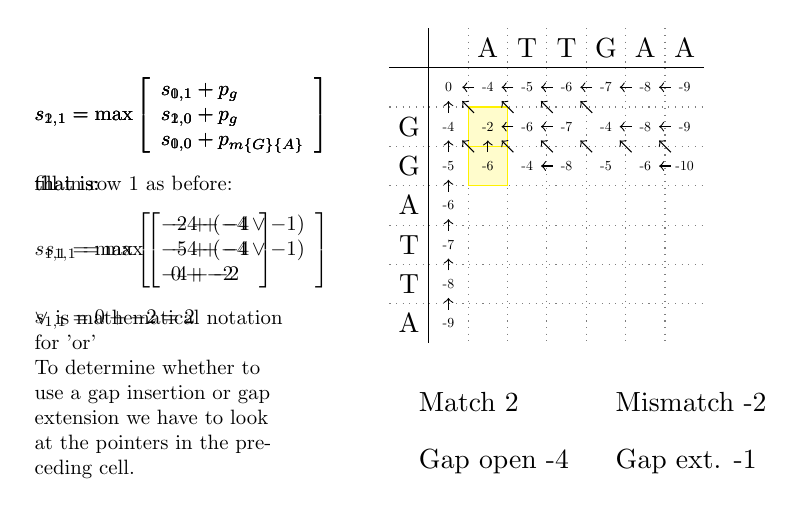
\begin{tikzpicture}[scale=0.5]
      \node [right] at (1,-1) {Match 2};
\node [right] at (6,-1) {Mismatch -2};
\node [right] at (1,-2.5) {Gap open -4};
\node [right] at (6,-2.5) {Gap ext. -1};
\visible<1->{
\draw [-] (0.5,7.5) -- (8.5,7.5);
\draw [-] (1.5,8.5) -- (1.5,0.5);
\draw [-, dotted, opacity=0.5] (0.5,6.5) -- (8.5,6.5);
\draw [-, dotted, opacity=0.5] (2.5,8.5) -- (2.5,0.5);
	\node at (3,8) {A};
	\draw [-, dotted, opacity=0.5] (3.5,8.5) -- (3.5,0.5);
	\node at (4,8) {T};
	\draw [-, dotted, opacity=0.5] (4.5,8.5) -- (4.5,0.5);
	\node at (5,8) {T};
	\draw [-, dotted, opacity=0.5] (5.5,8.5) -- (5.5,0.5);
	\node at (6,8) {G};
	\draw [-, dotted, opacity=0.5] (6.5,8.5) -- (6.5,0.5);
	\node at (7,8) {A};
	\draw [-, dotted, opacity=0.5] (7.5,8.5) -- (7.5,0.5);
	\node at (8,8) {A};
	\node at (1,6) {G};
	\draw [-, dotted, opacity=0.5] (0.5,5.5) -- (8.5,5.5);
	\node at (1,5) {G};
	\draw [-, dotted, opacity=0.5] (0.5,4.5) -- (8.5,4.5);
	\node at (1,4) {A};
	\draw [-, dotted, opacity=0.5] (0.5,3.5) -- (8.5,3.5);
	\node at (1,3) {T};
	\draw [-, dotted, opacity=0.5] (0.5,2.5) -- (8.5,2.5);
	\node at (1,2) {T};
	\draw [-, dotted, opacity=0.5] (0.5,1.5) -- (8.5,1.5);
	\node at (1,1) {A};
}

% \visible<2>{
% 	\node [below left, align=left, scale=0.75, text width=12em] 
% 	at (0,8) {1. Set up a matrix with each sequence 
% 	along an axis and with an empty row for each sequence.};
% }

\visible<1->{
	\node[scale=0.5] at (2,7) {0};
	\node[scale=0.5] at (3,7) {-4};
	\draw [->] (2.65, 6+1) -- (2.35, 6+1);
	\node[scale=0.5] at(4,7) {-5};
	\draw [->] (3.65,6+1) -- (3.35,6+1);
	\node[scale=0.5] at(5,7) {-6};
	\draw [->] (4.65,6+1) -- (4.35,6+1);
	\node[scale=0.5] at(6,7) {-7};
	\draw [->] (5.65,6+1) -- (5.35,6+1);
	\node[scale=0.5] at(7,7) {-8};
	\draw [->] (6.65,6+1) -- (6.35,6+1);
	\node[scale=0.5] at(8,7) {-9};
	\draw [->] (7.65,6+1) -- (7.35,6+1);
	\node[scale=0.5] at (2,6) {-4};
	\draw [->] (2,6 + 0.35) -- (2, 6 + 0.65);
	\node[scale=0.5] at(2,5) {-5};
	\draw [->] (2,6-1 + 0.35) -- (2, 6-1 + 0.65);
	\node[scale=0.5] at(2,4) {-6};
	\draw [->] (2,6-2 + 0.35) -- (2, 6-2 + 0.65);
	\node[scale=0.5] at(2,3) {-7};
	\draw [->] (2,6-3 + 0.35) -- (2, 6-3 + 0.65);
	\node[scale=0.5] at(2,2) {-8};
	\draw [->] (2,6-4 + 0.35) -- (2, 6-4 + 0.65);
	\node[scale=0.5] at(2,1) {-9};
	\draw [->] (2,6-5 + 0.35) -- (2, 6-5 + 0.65);
}

\visible<2-3>{
	\draw [fill, yellow, fill opacity=0.2] (2.5,5.5) rectangle (3.5,6.5);
	\node [below left, align=left, scale=0.75, text width=12em] 
	at (-2,8) 
	{
	$$
	s_{1,1} = \max
		\left[
		\begin{array}{l}
		s_{0,1} + p_g\\
		s_{1,0} + p_g\\
		s_{0,0} + p_{m\{G\}\{A\}}
		\end{array}
		\right]
	$$

	that is:
	$$
	s_{1,1} = \max
		\left[
		\begin{array}{l}
		-4 + -4\\
		-4 + -4\\
		0  + -2%
		\end{array}%
		\right]
	$$

	$s_{1,1} = 0 + -2 = 2$
	};
}


\visible<3->{
	\node [scale=0.5] at (3,6) {-2};
	\draw [->] (2.65,6.35) -- (2.35,6.65);
}

\visible<4>{
	\node [below left, align=left, scale=0.75, text width=12em] 
	at (-2,8) 
	{
	$$
	s_{1,1} = \max
		\left[
		\begin{array}{l}
		s_{0,1} + p_g\\
		s_{1,0} + p_g\\
		s_{0,0} + p_{m\{G\}\{A\}}
		\end{array}
		\right]
	$$

	fill in row 1 as before:
	};
}



\visible<4->{
	\node [scale=0.5] at (4,6) {-6};
	\draw [->] (3.65,6.35) -- (3.35,6.65);
	\draw [->] (3.65,6) -- (3.35,6);
	\node [scale=0.5] at (5,6) {-7};
	\draw [->] (4.65,6.35) -- (4.35,6.65);
	\draw [->] (4.65,6) -- (4.35,6);
	\node [scale=0.5] at (6,6) {-4};
	\draw [->] (5.65,6.35) -- (5.35,6.65);
	\node [scale=0.5] at (7,6) {-8};
	\draw [->] (6.65,6) -- (6.35,6);
	\node [scale=0.5] at (8,6) {-9};
	\draw [->] (7.65,6) -- (7.35,6);
}

% \visible<4>{
% 	\node [below left, align=left, scale=0.75, text width=12em] 
% 	at (0,8) {3. Determine the scores for individual cells progressing from
% 	the top left cell. The score $S_{i,j}$ at row $i$ and column $j$ is the max of:\\
% 	a) $S_{i-1,j-1} + P$\\
% 	{\footnotesize($P$ is $P_m$ or $P_{mm}$).
% 	}\\
% 	b) $S_{i,j-1} + P_{gap}$\\
% 	c) $S_{i-1,j} + P_{gap}$\\
% 	{\footnotesize $P_{gap}$ is either $P_{gip}$ or $P_{gop}$}\\
% 	\vspace{0.2cm}
% 	The path(s) giving the maximal score(s) is remembered and represented as
% 	an arrow.
% 	};
% }

\visible<5-6>{
 	\draw [fill, yellow, fill opacity=0.2] (2.5,4.5) rectangle (3.5,5.5);
	\node [below left, align=left, scale=0.75, text width=12em] 
	at (-2,8) 
	{
	$$
	s_{2,1} = \max
		\left[
		\begin{array}{l}
		s_{1,1} + p_g\\
		s_{2,0} + p_g\\
		s_{1,0} + p_{m\{G\}\{A\}}
		\end{array}
		\right]
	$$

	that is:
	$$
	s_{1,1} = \max
		\left[
		\begin{array}{l}
		-2 + (-4 \vee -1)\\
		-5 + (-4 \vee -1)\\
		-4  + -2%
		\end{array}%
		\right]
	$$
	$\vee$ is mathematical notation for 'or'\\

	To determine whether to use a gap insertion or gap extension we have
	to look at the pointers in the preceding cell.
	};	
}


\visible<6->{
	\node [scale=0.5] at (3,5) {-6};
	\draw [->] (2.65,5.35) -- (2.35,5.65);
}


\visible<7->{
% 	\node [scale=0.5] at (3,5) {-6};
% 	\draw [->] (2.65,5.35) -- (2.35,5.65);
	\draw [->] (3,5.35) -- (3,5.65);
	\node [scale=0.5] at (4,5) {-4};
	\draw [->] (3.65,5.35) -- (3.35,5.65);
	\node [scale=0.5] at (5,5) {-8};
	\draw [->] (4.65,5.35) -- (4.35,5.65);
	\draw [->] (4.65,5) -- (4.35,5);
	\node [scale=0.5] at (6,5) {-5};
	\draw [->] (5.65,5.35) -- (5.35,5.65);
	\node [scale=0.5] at (7,5) {-6};
	\draw [->] (6.65,5.35) -- (6.35,5.65);
	\node [scale=0.5] at (8,5) {-10};
	\draw [->] (7.65,5.35) -- (7.35,5.65);
	\draw [->] (7.65,5) -- (7.35,5);
}

% \visible<5>{
% 	\draw [fill, yellow, fill opacity=0.2] (2.5,4.5) rectangle (3.5,5.5);
% 	\node [below left, align=left, scale=0.75, text width=12em] 
% 	at (0,8) {
% 	The score at [3,2] (highlighted) is -6 as the score at [2,1] is -4, and there is a
% 	mismatch at [3,2] (G != A). 

% 	The score can also become -6 through a gap
% 	insertion from [2,2].
% 	};

% }

% \visible<6->{
% 	\node [scale=0.5] at (3,4) {-3};
% 	\draw [->] (2.65,4.35) -- (2.35,4.65);
% 	\node [scale=0.5] at (4,4) {-7};
% 	\draw [->] (3.65,4) -- (3.35,4);
% 	\node [scale=0.5] at (5,4) {-6};
% 	\draw [->] (4.65,4.35) -- (4.35,4.65);
% 	\node [scale=0.5] at (6,4) {-9};
% 	\draw [->] (6,4.35) -- (6,4.65);
% 	\node [scale=0.5] at (7,4) {-3};
% 	\draw [->] (6.65,4.35) -- (6.35,4.65);
% 	\node [scale=0.5] at (8,4) {-4};
% 	\draw [->] (7.65,4.35) -- (7.35,4.65);
% }
% \visible<7->{
% 	\node [scale=0.5] at (3,3) {-7};
% 	\draw [->] (3,3.35) -- (3,3.65);
% 	\node [scale=0.5] at (4,3) {-1};
% 	\draw [->] (3.65,3.35) -- (3.35,3.65);
% 	\node [scale=0.5] at (5,3) {-5};
% 	\draw [->] (4.65,3.35) -- (4.35,3.65);
% 	\draw [->] (4.65,3) -- (4.35,3);
% 	\node [scale=0.5] at (6,3) {-6};
% 	\draw [->] (5.65,3) -- (5.35,3);
% 	\node [scale=0.5] at (7,3) {-7};
% 	\draw [->] (6.65,3) -- (6.35,3);
% 	\draw [->] (7,3.35) -- (7,3.65);
% 	\node [scale=0.5] at (8,3) {-5};
% 	\draw [->] (7.65,3.35) -- (7.35,3.65);
% }
% \visible<8->{
% 	\node [scale=0.5] at (3,2) {-8};
% 	\draw [->] (3,2.35) -- (3,2.65);
% 	\node [scale=0.5] at (4,2) {-5};
% 	\draw [->] (3.65,2.35) -- (3.35,2.65);
% 	\draw [->] (4,2.35) -- (4,2.65);
% 	\node [scale=0.5] at (5,2) {1};
% 	\draw [->] (4.65,2.35) -- (4.35,2.65);
% 	\node [scale=0.5] at (6,2) {-3};
% 	\draw [->] (5.65,2) -- (5.35,2);
% 	\node [scale=0.5] at (7,2) {-4};
% 	\draw [->] (6.65,2) -- (6.35,2);
% 	\node [scale=0.5] at (8,2) {-5};
% 	\draw [->] (7.65,2) -- (7.35,2);
% }
% \visible<9->{
% 	\node [scale=0.5] at (3,1) {-6};
% 	\draw [->] (2.65,1.35) -- (2.35,1.65);
% 	\node [scale=0.5] at (4,1) {-6};
% 	\draw [->] (4,1.35) -- (4,1.65);
% 	\node [scale=0.5] at (5,1) {-3};
% 	\draw [->] (5,1.35) -- (5,1.65);
% 	\node [scale=0.5] at (6,1) {-1};
% 	\draw [->] (5.65,1.35) -- (5.35,1.65);
% 	\node [scale=0.5] at (7,1) {-1};
% 	\draw [->] (6.65,1.35) -- (6.35,1.65);
% 	\node [scale=0.5] at (8,1) {-2};
% 	\draw [->] (7.65,1.35) -- (7.35,1.65);
% }
% \visible<10->{
% \draw [fill=yellow, fill opacity=0.1] (7.5,0.5) rectangle (8.5,1.5);
% }
% \visible<11->{
% \draw [fill=yellow, fill opacity=0.1] (6.5,1.5) rectangle (7.5,2.5);
% }
% \visible<12->{
% \draw [fill=yellow, fill opacity=0.1] (5.5,1.5) rectangle (6.5,2.5);
% }
% \visible<13->{
% \draw [fill=yellow, fill opacity=0.1] (4.5,1.5) rectangle (5.5,2.5);
% }
% \visible<14->{
% \draw [fill=yellow, fill opacity=0.1] (3.5,2.5) rectangle (4.5,3.5);
% }
% \visible<15->{
% \draw [fill=yellow, fill opacity=0.1] (2.5,3.5) rectangle (3.5,4.5);
% }
% \visible<16->{
% \draw [fill=yellow, fill opacity=0.1] (1.5,4.5) rectangle (2.5,5.5);
% }
% \visible<17->{
% \draw [fill=yellow, fill opacity=0.1] (1.5,5.5) rectangle (2.5,6.5);
% }
% \visible<18->{
% \draw [fill=yellow, fill opacity=0.1] (1.5,6.5) rectangle (2.5,7.5);
% }

% \visible<10-18>{
% 	\node [below left, align=left, scale=0.75, text width=12em] 
% 	at (0,8) {
% 	Follow the path (arrows) from the bottom right to
% 	the top left corner.

% 	Diagonal movements insert a letter from both sequences,
% 	left or upwards insert a letter and a gap.
% 	};
% }

% \visible<19->{
% \node [scale=0.75] (s1) at (10 + 0/2.5, 5) {-};
% \node [scale=0.75] (s2) at (10 + 0/2.5, 5-1.25) {G};
% \node [scale=0.75] (s1) at (10 + 1/2.5, 5) {-};
% \node [scale=0.75] (s2) at (10 + 1/2.5, 5-1.25) {G};
% \node [scale=0.75] (s1) at (10 + 2/2.5, 5) {A};
% \node [scale=0.75] (s2) at (10 + 2/2.5, 5-1.25) {A};
% \draw [-] (s1) -- (s2);
% \node [scale=0.75] (s1) at (10 + 3/2.5, 5) {T};
% \node [scale=0.75] (s2) at (10 + 3/2.5, 5-1.25) {T};
% \draw [-] (s1) -- (s2);
% \node [scale=0.75] (s1) at (10 + 4/2.5, 5) {T};
% \node [scale=0.75] (s2) at (10 + 4/2.5, 5-1.25) {T};
% \draw [-] (s1) -- (s2);
% \node [scale=0.75] (s1) at (10 + 5/2.5, 5) {G};
% \node [scale=0.75] (s2) at (10 + 5/2.5, 5-1.25) {-};
% \node [scale=0.75] (s1) at (10 + 6/2.5, 5) {A};
% \node [scale=0.75] (s2) at (10 + 6/2.5, 5-1.25) {-};
% \node [scale=0.75] (s1) at (10 + 7/2.5, 5) {A};
% \node [scale=0.75] (s2) at (10 + 7/2.5, 5-1.25) {A};
% \draw [-] (s1) -- (s2);
% }

    \end{tikzpicture}
  \end{figure}
\end{frame}

\begin{frame}[fragile]{Scoring}
  \begin{columns}
    \begin{column}{0.6\textwidth}
      \begin{perlcode}
        sub score_cell {
          my ($i, $j) = @_;
        ## make three different scores
        ## for the different alternatives
        my $sc_1 = $scores[$i-1][$j] + gp($i,$j,1);
        my $sc_2 = $scores[$i][$j-1] + gp($i,$j,2);
        my $sc_2 = $scores[$i-1][$j-1] +
                   $matrix{ $seq1[$i-1] }{ $seq[$j-1] };
        
        ## find the max score and set the
        ## score and the pointer tables
        ($scores[$i][$j], $pointers[$i][$j]) =
                max_score($sc_1, $sc_2, $sc_3);
        }
      \end{perlcode}
    \end{column}
    \begin{column}{0.4\textwidth}
      \begin{figure}[ht]
        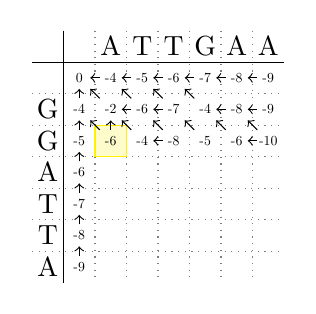
\begin{tikzpicture}[scale=0.4]
          % \node [right, scale=0.5] at (1,-1) {Match 2};
% \node [right, scale=] at (6,-1) {Mismatch -2};
% \node [right] at (1,-2.5) {Gap open -4};
% \node [right] at (6,-2.5) {Gap ext. -1};

\visible<1->{
\draw [-] (0.5,7.5) -- (8.5,7.5);
\draw [-] (1.5,8.5) -- (1.5,0.5);
\draw [-, dotted, opacity=0.5] (0.5,6.5) -- (8.5,6.5);
\draw [-, dotted, opacity=0.5] (2.5,8.5) -- (2.5,0.5);
	\node at (3,8) {A};
	\draw [-, dotted, opacity=0.5] (3.5,8.5) -- (3.5,0.5);
	\node at (4,8) {T};
	\draw [-, dotted, opacity=0.5] (4.5,8.5) -- (4.5,0.5);
	\node at (5,8) {T};
	\draw [-, dotted, opacity=0.5] (5.5,8.5) -- (5.5,0.5);
	\node at (6,8) {G};
	\draw [-, dotted, opacity=0.5] (6.5,8.5) -- (6.5,0.5);
	\node at (7,8) {A};
	\draw [-, dotted, opacity=0.5] (7.5,8.5) -- (7.5,0.5);
	\node at (8,8) {A};
	\node at (1,6) {G};
	\draw [-, dotted, opacity=0.5] (0.5,5.5) -- (8.5,5.5);
	\node at (1,5) {G};
	\draw [-, dotted, opacity=0.5] (0.5,4.5) -- (8.5,4.5);
	\node at (1,4) {A};
	\draw [-, dotted, opacity=0.5] (0.5,3.5) -- (8.5,3.5);
	\node at (1,3) {T};
	\draw [-, dotted, opacity=0.5] (0.5,2.5) -- (8.5,2.5);
	\node at (1,2) {T};
	\draw [-, dotted, opacity=0.5] (0.5,1.5) -- (8.5,1.5);
	\node at (1,1) {A};
}


\visible<1->{
	\node[scale=0.5] at (2,7) {0};
	\node[scale=0.5] at (3,7) {-4};
	\draw [->] (2.65, 6+1) -- (2.35, 6+1);
	\node[scale=0.5] at(4,7) {-5};
	\draw [->] (3.65,6+1) -- (3.35,6+1);
	\node[scale=0.5] at(5,7) {-6};
	\draw [->] (4.65,6+1) -- (4.35,6+1);
	\node[scale=0.5] at(6,7) {-7};
	\draw [->] (5.65,6+1) -- (5.35,6+1);
	\node[scale=0.5] at(7,7) {-8};
	\draw [->] (6.65,6+1) -- (6.35,6+1);
	\node[scale=0.5] at(8,7) {-9};
	\draw [->] (7.65,6+1) -- (7.35,6+1);
	\node[scale=0.5] at (2,6) {-4};
	\draw [->] (2,6 + 0.35) -- (2, 6 + 0.65);
	\node[scale=0.5] at(2,5) {-5};
	\draw [->] (2,6-1 + 0.35) -- (2, 6-1 + 0.65);
	\node[scale=0.5] at(2,4) {-6};
	\draw [->] (2,6-2 + 0.35) -- (2, 6-2 + 0.65);
	\node[scale=0.5] at(2,3) {-7};
	\draw [->] (2,6-3 + 0.35) -- (2, 6-3 + 0.65);
	\node[scale=0.5] at(2,2) {-8};
	\draw [->] (2,6-4 + 0.35) -- (2, 6-4 + 0.65);
	\node[scale=0.5] at(2,1) {-9};
	\draw [->] (2,6-5 + 0.35) -- (2, 6-5 + 0.65);
}


\visible<1->{
	\node [scale=0.5] at (3,6) {-2};
	\draw [->] (2.65,6.35) -- (2.35,6.65);
}


\visible<1->{
	\node [scale=0.5] at (4,6) {-6};
	\draw [->] (3.65,6.35) -- (3.35,6.65);
	\draw [->] (3.65,6) -- (3.35,6);
	\node [scale=0.5] at (5,6) {-7};
	\draw [->] (4.65,6.35) -- (4.35,6.65);
	\draw [->] (4.65,6) -- (4.35,6);
	\node [scale=0.5] at (6,6) {-4};
	\draw [->] (5.65,6.35) -- (5.35,6.65);
	\node [scale=0.5] at (7,6) {-8};
	\draw [->] (6.65,6) -- (6.35,6);
	\node [scale=0.5] at (8,6) {-9};
	\draw [->] (7.65,6) -- (7.35,6);
}


\visible<1->{
 	\draw [fill, yellow, fill opacity=0.2] (2.5,4.5) rectangle (3.5,5.5);
}


\visible<1->{
	\node [scale=0.5] at (3,5) {-6};
	\draw [->] (2.65,5.35) -- (2.35,5.65);
}


\visible<2->{
% 	\node [scale=0.5] at (3,5) {-6};
% 	\draw [->] (2.65,5.35) -- (2.35,5.65);
	\draw [->] (3,5.35) -- (3,5.65);
	\node [scale=0.5] at (4,5) {-4};
	\draw [->] (3.65,5.35) -- (3.35,5.65);
	\node [scale=0.5] at (5,5) {-8};
	\draw [->] (4.65,5.35) -- (4.35,5.65);
	\draw [->] (4.65,5) -- (4.35,5);
	\node [scale=0.5] at (6,5) {-5};
	\draw [->] (5.65,5.35) -- (5.35,5.65);
	\node [scale=0.5] at (7,5) {-6};
	\draw [->] (6.65,5.35) -- (6.35,5.65);
	\node [scale=0.5] at (8,5) {-10};
	\draw [->] (7.65,5.35) -- (7.35,5.65);
	\draw [->] (7.65,5) -- (7.35,5);
}

% \visible<5>{
% 	\draw [fill, yellow, fill opacity=0.2] (2.5,4.5) rectangle (3.5,5.5);
% 	\node [below left, align=left, scale=0.75, text width=12em] 
% 	at (0,8) {
% 	The score at [3,2] (highlighted) is -6 as the score at [2,1] is -4, and there is a
% 	mismatch at [3,2] (G != A). 

% 	The score can also become -6 through a gap
% 	insertion from [2,2].
% 	};

% }

% \visible<6->{
% 	\node [scale=0.5] at (3,4) {-3};
% 	\draw [->] (2.65,4.35) -- (2.35,4.65);
% 	\node [scale=0.5] at (4,4) {-7};
% 	\draw [->] (3.65,4) -- (3.35,4);
% 	\node [scale=0.5] at (5,4) {-6};
% 	\draw [->] (4.65,4.35) -- (4.35,4.65);
% 	\node [scale=0.5] at (6,4) {-9};
% 	\draw [->] (6,4.35) -- (6,4.65);
% 	\node [scale=0.5] at (7,4) {-3};
% 	\draw [->] (6.65,4.35) -- (6.35,4.65);
% 	\node [scale=0.5] at (8,4) {-4};
% 	\draw [->] (7.65,4.35) -- (7.35,4.65);
% }
% \visible<7->{
% 	\node [scale=0.5] at (3,3) {-7};
% 	\draw [->] (3,3.35) -- (3,3.65);
% 	\node [scale=0.5] at (4,3) {-1};
% 	\draw [->] (3.65,3.35) -- (3.35,3.65);
% 	\node [scale=0.5] at (5,3) {-5};
% 	\draw [->] (4.65,3.35) -- (4.35,3.65);
% 	\draw [->] (4.65,3) -- (4.35,3);
% 	\node [scale=0.5] at (6,3) {-6};
% 	\draw [->] (5.65,3) -- (5.35,3);
% 	\node [scale=0.5] at (7,3) {-7};
% 	\draw [->] (6.65,3) -- (6.35,3);
% 	\draw [->] (7,3.35) -- (7,3.65);
% 	\node [scale=0.5] at (8,3) {-5};
% 	\draw [->] (7.65,3.35) -- (7.35,3.65);
% }
% \visible<8->{
% 	\node [scale=0.5] at (3,2) {-8};
% 	\draw [->] (3,2.35) -- (3,2.65);
% 	\node [scale=0.5] at (4,2) {-5};
% 	\draw [->] (3.65,2.35) -- (3.35,2.65);
% 	\draw [->] (4,2.35) -- (4,2.65);
% 	\node [scale=0.5] at (5,2) {1};
% 	\draw [->] (4.65,2.35) -- (4.35,2.65);
% 	\node [scale=0.5] at (6,2) {-3};
% 	\draw [->] (5.65,2) -- (5.35,2);
% 	\node [scale=0.5] at (7,2) {-4};
% 	\draw [->] (6.65,2) -- (6.35,2);
% 	\node [scale=0.5] at (8,2) {-5};
% 	\draw [->] (7.65,2) -- (7.35,2);
% }
% \visible<9->{
% 	\node [scale=0.5] at (3,1) {-6};
% 	\draw [->] (2.65,1.35) -- (2.35,1.65);
% 	\node [scale=0.5] at (4,1) {-6};
% 	\draw [->] (4,1.35) -- (4,1.65);
% 	\node [scale=0.5] at (5,1) {-3};
% 	\draw [->] (5,1.35) -- (5,1.65);
% 	\node [scale=0.5] at (6,1) {-1};
% 	\draw [->] (5.65,1.35) -- (5.35,1.65);
% 	\node [scale=0.5] at (7,1) {-1};
% 	\draw [->] (6.65,1.35) -- (6.35,1.65);
% 	\node [scale=0.5] at (8,1) {-2};
% 	\draw [->] (7.65,1.35) -- (7.35,1.65);
% }
% \visible<10->{
% \draw [fill=yellow, fill opacity=0.1] (7.5,0.5) rectangle (8.5,1.5);
% }
% \visible<11->{
% \draw [fill=yellow, fill opacity=0.1] (6.5,1.5) rectangle (7.5,2.5);
% }
% \visible<12->{
% \draw [fill=yellow, fill opacity=0.1] (5.5,1.5) rectangle (6.5,2.5);
% }
% \visible<13->{
% \draw [fill=yellow, fill opacity=0.1] (4.5,1.5) rectangle (5.5,2.5);
% }
% \visible<14->{
% \draw [fill=yellow, fill opacity=0.1] (3.5,2.5) rectangle (4.5,3.5);
% }
% \visible<15->{
% \draw [fill=yellow, fill opacity=0.1] (2.5,3.5) rectangle (3.5,4.5);
% }
% \visible<16->{
% \draw [fill=yellow, fill opacity=0.1] (1.5,4.5) rectangle (2.5,5.5);
% }
% \visible<17->{
% \draw [fill=yellow, fill opacity=0.1] (1.5,5.5) rectangle (2.5,6.5);
% }
% \visible<18->{
% \draw [fill=yellow, fill opacity=0.1] (1.5,6.5) rectangle (2.5,7.5);
% }

% \visible<10-18>{
% 	\node [below left, align=left, scale=0.75, text width=12em] 
% 	at (0,8) {
% 	Follow the path (arrows) from the bottom right to
% 	the top left corner.

% 	Diagonal movements insert a letter from both sequences,
% 	left or upwards insert a letter and a gap.
% 	};
% }

% \visible<19->{
% \node [scale=0.75] (s1) at (10 + 0/2.5, 5) {-};
% \node [scale=0.75] (s2) at (10 + 0/2.5, 5-1.25) {G};
% \node [scale=0.75] (s1) at (10 + 1/2.5, 5) {-};
% \node [scale=0.75] (s2) at (10 + 1/2.5, 5-1.25) {G};
% \node [scale=0.75] (s1) at (10 + 2/2.5, 5) {A};
% \node [scale=0.75] (s2) at (10 + 2/2.5, 5-1.25) {A};
% \draw [-] (s1) -- (s2);
% \node [scale=0.75] (s1) at (10 + 3/2.5, 5) {T};
% \node [scale=0.75] (s2) at (10 + 3/2.5, 5-1.25) {T};
% \draw [-] (s1) -- (s2);
% \node [scale=0.75] (s1) at (10 + 4/2.5, 5) {T};
% \node [scale=0.75] (s2) at (10 + 4/2.5, 5-1.25) {T};
% \draw [-] (s1) -- (s2);
% \node [scale=0.75] (s1) at (10 + 5/2.5, 5) {G};
% \node [scale=0.75] (s2) at (10 + 5/2.5, 5-1.25) {-};
% \node [scale=0.75] (s1) at (10 + 6/2.5, 5) {A};
% \node [scale=0.75] (s2) at (10 + 6/2.5, 5-1.25) {-};
% \node [scale=0.75] (s1) at (10 + 7/2.5, 5) {A};
% \node [scale=0.75] (s2) at (10 + 7/2.5, 5-1.25) {A};
% \draw [-] (s1) -- (s2);
% }

        \end{tikzpicture}
      \end{figure}
      \end{column}
  \end{columns}
  
  \pause
  \pause
  \footnotesize{
  We calculate the three alternative scores which represent the two different
  gap insertions (in either sequence) or an aligned pair.

  We have to decide whether a gap insertion or gap extension penalty is
  appropriate. Not sure of the best way to do this, so we pretend that we have
  defined a function that will do this for us.

  Similarly we have to find the maximum score and think of a way of defining
  the pointer table. Again we postpone this work; we'll make another function
  in the future that takes care of the problem.

  }
\end{frame}


\begin{frame}[fragile]{The pointers?}
  We need to have a table that remembers the pointers. That is we need some
  way to encode:

  \begin{itemize}
    \item up
    \item left
    \item up \& left
  \end{itemize}
  
  And any combination of the above (in theory we can have all three pointers
  from a cell; this will happen if all three paths give the same score).

  How??
\end{frame}

\begin{frame}[fragile]{Think binary}
  Consider if we decide to encode using numbers that are even powers of two
  then we can say:

  \begin{description}
  \item[0] No pointer (needed for Smith-Waterman)
  \item[1] Up
  \item[2] Left
  \item[4] Up/Left (i.e. diagonal)
  \end{description}
  
  Then hopefully you can see that the sum of all specific combinations give
  unique values. That is we can use a single number to encode any combination
  of the pointers.
\end{frame}

\begin{frame}[fragile]{How do we use this?}
  \small{
  Consider how 0, 1, 2, and 4 are encoded in binary:

  \begin{tabular}{ c|cccc }
    d & 4 & 2 & 1\\
    \hline
    0 & 0 & 0 & 0\\
    1 & 0 & 0 & 1\\
    2 & 0 & 1 & 0\\
    4 & 1 & 0 & 0
  \end{tabular}

  We can consider numbers between 0 and 7 (1 + 2 + 4) to consist of 3
  individual bits, with 0 = 000, 7 = 111.\\
  
  \pause
  \vspace{0.5cm}
  In the suggested scoring scheme:

  \begin{tabular}{ c|cccc }
    ptr & 4 & 2 & 1\\
    \hline
    no & 0 & 0 & 0\\
    up & 0 & 0 & 1\\
    left & 0 & 1 & 0\\
    diagonal & 1 & 0 & 0
  \end{tabular}
  }
\end{frame}

\begin{frame}[fragile]{Encoding \& Decoding}
  To encode a pointer use bitwise \texttt{OR} operator \verb#|#.
  
  \begin{tabular}{ c|ccc|c }
    1 & 0 & 0 & 1 &\\
    2 & 0 & 1 & 0 & OR\\
    \hline
    3 & 0 & 1 & 1 &\\
  \end{tabular}
  
  \vspace{0.5cm}
  To decode a pointer use bitwise \texttt{AND} operator \verb|&|.\\
  \begin{tabular}{ c|ccc|c }
    2 & 0 & 1 & 0 &\\
    3 & 0 & 1 & 1 & AND\\
    \hline
    2 & 0 & 1 & 0 &\\
  \end{tabular}
  
  \vspace{0.5cm}
  in perl:
  \begin{perlcode}
    $a = 1 | 2;
    $b = 2 & 3;

    ## $a is now 3, and $b is 2
  \end{perlcode}
\end{frame}

\begin{frame}[fragile]{That \texttt{max\_score()} function}
  We proposed using a \texttt{max\_score()} function to determine both the max
  score and to set the pointer. We define this function as taking three
  arguments:
  \begin{enumerate}
  \item UP score
  \item LEFT score
  \item DIAGONAL score
  \end{enumerate}
  
  Remember that these are delivered to the function in the \verb|@_| array:

  \begin{perlcode}
    sub max_score {
      my $max = $_[0];
      for my $i(1..$#_){
        if( $max < $_[$i] ){ $max = $_[$i] };
      }
      my $ptr = 0;
      if( $_[0] == $max ){ $ptr = $ptr | 1; }
      if( $_[1] == $max ){ $ptr = $ptr | 2; }
      if( $_[2] == $max ){ $ptr = $ptr | 4; }
      return( $max, $ptr );
    }
  \end{perlcode}
\end{frame}

\begin{frame}[fragile]{and that \texttt{gp()} function}
  \texttt{gp()} is a function that determines whether a gap should be
  considered as a gap insertion or extension.

  To be lazy it will make use of the global \verb|$gap_open|,
  \verb|$gap_extend| and \verb|%pointer| variables. The function takes three arguments:

  \begin{enumerate}
  \item The row number 
  \item The column number
  \item Which parental cell is being considered
  \end{enumerate}
  
  \begin{perlcode}
    sub gp {
      my( $i, $j, $d ) = @_;
      ## if $d is 1 then we are looking up
      if( $d == 1 && $pointers[$i-1][$j] & $d ){ return($gap_extend); }
      if( $d == 2 && $pointers[$i][$j-1] & $d ){ return($gap_extend); }
      return( $gap_open )
    }
  \end{perlcode}
   
  For this function to work correctly it must receive the correct
  arguments. It cannot check them to make sure, so it has to be used with care.
\end{frame}

\begin{frame}[fragile]{Tracing back the alignment}
  Once we have completed the score table we need to trace back the best
  alignment.

  This is easy if we want to do it for every maximally scoring alignment.

  For now assume there is a function that returns a set of alignments:

  \begin{perlcode}
    @aligns = traceback();
  \end{perlcode}
  
  If we have time we will discuss:
\end{frame}

\begin{frame}[fragile]{Putting it together}
  \begin{perlcode}
    #!/usr/bin/perl
    use warnings;
    
    ($sfile1, $sfile2, $mfile, $gap_open, $gap_extend) = @ARGV;

    $seq1 = read_fasta($sfile1);
    $seq2 = read_fasta($sfile2);
    %matrix = read_matrix($mfile);

    init_tables(length($seq1), length($seq2), $gap_open, $gap_extend);
    
    ## then simpy go through and set up the scores:
    for($i=0; $i < length($seq1); $i++){
      for($j=0; $j < length($seq2): $j++){
        score_cell( $i+1, $j+1 );
      }
    }
    
    @aligns = traceback();
    
    ## and then the function definitions that we worked out elsewhere..
    ## ....
  \end{perlcode}
\end{frame}

\begin{frame}[fragile]{A recursive traceback function}
  \begin{perlcode}
    sub traceback {
      ## $al_ref is a reference to an array of strings
      ## The function pushes its $cigar to this when 
      ## it has a 0 pointer.. 
      my ($al_ref, $cigar, $i, $j) = @_;
      if( $pointers[$i][$j] == 0 ){
        push @{$al_ref}, $cigar;
        return;
      }
      if( $pointers[$i][$j] & 1 ){
        traceback($al_ref, 'I'.$cigar, $i-1, $j);
      }
      if( $pointers[$i][$j] & 2){
        traceback($al_ref, 'D'.$cigar, $i, $j-1);
      }
      if( $pointers[$i][$j] & 4){
        traceback($al_ref, 'M'.$cigar, $i-1, $j-1);
      }
    }
  \end{perlcode}

  \small A recursive function is a function that calls itself. This leads to
  'interesting behaviour', but is sometimes very useful.

  \small Here we call the function from the main body, with the coordinates of
  the starting (i.e. last cell) and trace our way back through the matrix.
\end{frame}

\begin{frame}[fragile]{Visualising the score table}
  \small We can use the SVG module to draw the alignment matrix to a .svg file
  which contains scalable vector graphics.

  \begin{figure}[ht]
    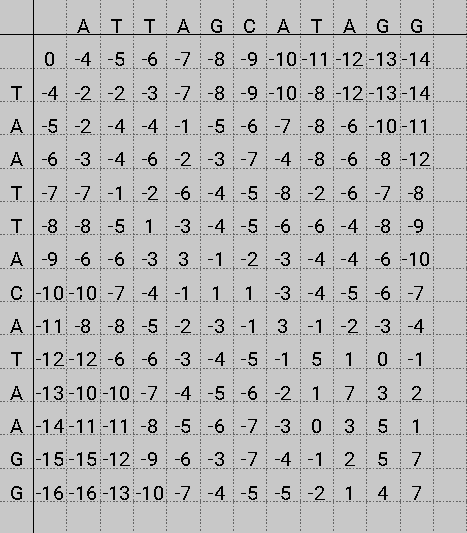
\includegraphics[width=0.5\textwidth]{images/scoreMatrix}
  \end{figure}
\end{frame}

\begin{frame}[fragile]{Graphical output}
  
  \small In the main body you'll need to add:
  \begin{perlcode}
    #!/usr/bin/perl
    use warnings;
    use SVG;
  \end{perlcode}

  Then the function. Which takes one argument: the file name of the svg output.

  \begin{perlcode}
  sub drawScoreTable {
    my ($filename) = @_;
    ## some constants that we should make into optional arguments
    my $char_width = 20;
    my $line_height = 20;
    my $line_offset = 1;  ## draw the lines below the characters
    
    my $height = ($#seq1 + 3) * $line_height + $char_width;
    my $width = ($#seq2 + 3) * $char_width + $char_width;
    
    ## draw a rect to have a background
    my $bg_color = 'rgb(200, 200, 200)';
    my $svg = SVG->new(width=>$width, height=>$height);
    
    $svg->rect(x=>0, y=>0, width=>$width, height=>$height, fill=>$bg_color);

  \end{perlcode}
  
  \tiny continued on next slide
\end{frame}

\begin{frame}[fragile]{Graphical output}
  \begin{perlcode}
    ## draw the sequences
    for my $i(0..$#seq1){
	$svg->text(x=>$char_width/2, y=>((3 + $i) * $line_height), 
        'text-anchor'=>'middle')->cdata($seq1[$i]);
    }
    for my $i(0..$#seq2){
	$svg->text(x=>(2.5 + $i)*$char_width, y=>$line_height, 
        'text-anchor'=>'middle')->cdata($seq2[$i]);
    }
    ## and lets draw a couple of lines
    $svg->line(x1=>$char_width, y1=>$height, 
               x2=>$char_width, y2=>0, stroke=>'rgb(0,0,0)', 'stroke-width'=>'0.5');
    $svg->line(x1=>0, y1=>$line_height+$line_offset, 
               x2=>$width, y2=>$line_height+$line_offset,
               stroke=>'rgb(0,0,0)', 
               'stroke-width'=>'0.5');

    ## and a few more ones:
    for my $i(0..@seq1){
      $svg->line(x1=>0, y1=>($i + 2) * $line_height + $line_offset, x2=>$width, 
      y2=>($i + 2) * $line_height +$line_offset, stroke=>'rgb(0,0,0)', 
      'stroke-width'=>'0.5', 'stroke-opacity'=>0.5, 'stroke-dasharray'=>(1));
    }
    for my $i(0..@seq1){
      $svg->line(x1=>(1 + $i) * $char_width, y1=>0, x2=>(1 + $i) * $char_width, y2=>$height,
      stroke=>'rgb(0,0,0)', 
      'stroke-width'=>'0.5', 'stroke-opacity'=>0.5, 'stroke-dasharray'=>(1));
    }
  \end{perlcode}
  \tiny continued on next slide    
\end{frame}

\begin{frame}[fragile]{Graphical output}
  \begin{perlcode}
    for my $i(0..$#scores){
      for my $j(0..$#{$scores[$i]}){
	$svg->text( x=>($char_width * 1.5 + $j * $char_width), 
              y=>(2 + $i) * $line_height, 
              'text-anchor'=>'middle')->cdata($scores[$i][$j]);
      }
    }
    
    my $xml = $svg->xmlify;
    open(my $out, ">", $filename) || die "unable to open $filename $!\n";
    print $out $xml;
    close $out;
  }
  \end{perlcode}
\end{frame}


\end{document}
